% appendix/whymb/whymemorybarriers.tex

\QuickQuizChapter{chp:app:whymb:Why Memory Barriers?}{Why Memory Barriers?}

So what possessed CPU designers to cause them to inflict memory barriers
on poor unsuspecting SMP software designers?

In short, because reordering memory references allows much better performance,
and so memory barriers are needed to force ordering in things like
synchronization primitives whose correct operation depends on ordered
memory references.

Getting a more detailed answer to this question requires a good understanding
of how CPU caches work, and especially what is required to make
caches really work well.
The following sections:
\begin{enumerate}
\item	present the structure of a cache,
\item	describe how cache-coherency protocols ensure that CPUs agree
	on the value of each location in memory, and, finally,
\item	outline how store buffers and invalidate queues help
	caches and cache-coherency protocols achieve high performance.
\end{enumerate}
We will see that memory barriers are a necessary evil that is required
to enable good performance and scalability, an evil that stems from
the fact that CPUs are orders of magnitude faster than are both the
interconnects between them and the memory they are attempting to access.

\section{Cache Structure}
\label{sec:app:whymb:Cache Structure}

Modern CPUs are much faster than are modern memory systems.
A 2006 CPU might be capable of executing ten instructions per nanosecond,
but will require many tens of nanoseconds to fetch a data item from
main memory.
This disparity in speed --- more than two orders of magnitude --- has
resulted in the multi-megabyte caches found on modern CPUs.
These caches are associated with the CPUs as shown in
Figure~\ref{fig:app:whymb:Modern Computer System Cache Structure},
and can typically be accessed in a few cycles.\footnote{
	It is standard practice to use multiple levels of cache,
	with a small level-one cache close to the CPU with
	single-cycle access time, and a larger level-two cache
	with a longer access time, perhaps roughly ten clock cycles.
	Higher-performance CPUs often have three or even four levels
	of cache.}

\begin{figure}[htb]
\begin{center}
\resizebox{3in}{!}{\includegraphics{appendix/whymb/cacheSC}}
\end{center}
\caption{Modern Computer System Cache Structure}
\label{fig:app:whymb:Modern Computer System Cache Structure}
\end{figure}

Data flows among the CPUs' caches and memory in fixed-length blocks
called ``cache lines'', which are normally a power of two in size,
ranging from 16 to 256 bytes.
When a given data item is first accessed by a given CPU, it will
be absent from that CPU's cache, meaning that a ``cache miss''
(or, more specifically, a ``startup'' or ``warmup'' cache miss)
has occurred.
The cache miss means that the CPU will
have to wait (or be ``stalled'') for hundreds of cycles while the
item is fetched from memory.
However, the item will be loaded into that CPU's cache, so that
subsequent accesses will find it in the cache and therefore run
at full speed.

After some time, the CPU's cache will fill, and subsequent
misses will likely need to eject an item from the cache in order
to make room for the newly fetched item.
Such a cache miss is termed a ``capacity miss'', because it is caused
by the cache's limited capacity.
However, most caches can be forced to eject an old item to make room
for a new item even when they are not yet full.
This is due to the fact that large caches are implemented as hardware
hash tables with fixed-size hash buckets (or ``sets'', as CPU designers
call them) and no chaining, as shown in
Figure~\ref{fig:app:whymb:CPU Cache Structure}.

This cache has sixteen ``sets'' and two ``ways'' for a total of 32
``lines'', each entry containing a single 256-byte ``cache line'',
which is a 256-byte-aligned block of memory.
This cache line size is a little on the large size, but makes the hexadecimal
arithmetic much simpler.
In hardware parlance, this is a two-way set-associative cache, and
is analogous to a software hash table with
sixteen buckets, where each bucket's hash chain is limited to
at most two elements.
The size (32 cache lines in this case) and the associativity (two in
this case) are collectively called the cache's ``geometry''.
Since this cache is implemented in hardware, the hash function is
extremely simple: extract four bits from the memory address.

\begin{figure}[t]
\begin{center}
\small
\begin{picture}(170,170)(0,0)

	% Addresses

	\put(0,0){\makebox(20,10){\tt 0xF}}
	\put(0,10){\makebox(20,10){\tt 0xE}}
	\put(0,20){\makebox(20,10){\tt 0xD}}
	\put(0,30){\makebox(20,10){\tt 0xC}}
	\put(0,40){\makebox(20,10){\tt 0xB}}
	\put(0,50){\makebox(20,10){\tt 0xA}}
	\put(0,60){\makebox(20,10){\tt 0x9}}
	\put(0,70){\makebox(20,10){\tt 0x8}}
	\put(0,80){\makebox(20,10){\tt 0x7}}
	\put(0,90){\makebox(20,10){\tt 0x6}}
	\put(0,100){\makebox(20,10){\tt 0x5}}
	\put(0,110){\makebox(20,10){\tt 0x4}}
	\put(0,120){\makebox(20,10){\tt 0x3}}
	\put(0,130){\makebox(20,10){\tt 0x2}}
	\put(0,140){\makebox(20,10){\tt 0x1}}
	\put(0,150){\makebox(20,10){\tt 0x0}}

	% Way 0

	\put(20,163){\makebox(80,10){Way 0}}
	\put(20,0){\framebox(80,10){\tt }}
	\put(20,10){\framebox(80,10){\tt 0x12345E00}}
	\put(20,20){\framebox(80,10){\tt 0x12345D00}}
	\put(20,30){\framebox(80,10){\tt 0x12345C00}}
	\put(20,40){\framebox(80,10){\tt 0x12345B00}}
	\put(20,50){\framebox(80,10){\tt 0x12345A00}}
	\put(20,60){\framebox(80,10){\tt 0x12345900}}
	\put(20,70){\framebox(80,10){\tt 0x12345800}}
	\put(20,80){\framebox(80,10){\tt 0x12345700}}
	\put(20,90){\framebox(80,10){\tt 0x12345600}}
	\put(20,100){\framebox(80,10){\tt 0x12345500}}
	\put(20,110){\framebox(80,10){\tt 0x12345400}}
	\put(20,120){\framebox(80,10){\tt 0x12345300}}
	\put(20,130){\framebox(80,10){\tt 0x12345200}}
	\put(20,140){\framebox(80,10){\tt 0x12345100}}
	\put(20,150){\framebox(80,10){\tt 0x12345000}}

	% Way 1

	\put(100,163){\makebox(80,10){Way 1}}
	\put(100,0){\framebox(80,10){\tt }}
	\put(100,10){\framebox(80,10){\tt 0x43210E00}}
	\put(100,20){\framebox(80,10){\tt }}
	\put(100,30){\framebox(80,10){\tt }}
	\put(100,40){\framebox(80,10){\tt }}
	\put(100,50){\framebox(80,10){\tt }}
	\put(100,60){\framebox(80,10){\tt }}
	\put(100,70){\framebox(80,10){\tt }}
	\put(100,80){\framebox(80,10){\tt }}
	\put(100,90){\framebox(80,10){\tt }}
	\put(100,100){\framebox(80,10){\tt }}
	\put(100,110){\framebox(80,10){\tt }}
	\put(100,120){\framebox(80,10){\tt }}
	\put(100,130){\framebox(80,10){\tt }}
	\put(100,140){\framebox(80,10){\tt }}
	\put(100,150){\framebox(80,10){\tt }}

\end{picture}
\end{center}
\caption{CPU Cache Structure}
\label{fig:app:whymb:CPU Cache Structure}
\end{figure}

In Figure~\ref{fig:app:whymb:CPU Cache Structure},
each box corresponds to a cache entry, which
can contain a 256-byte cache line.
However, a cache entry can be empty, as indicated by the empty boxes
in the figure.
The rest of the boxes are flagged with the memory address of the cache line
that they contain.
Since the cache lines must be 256-byte aligned, the low eight bits of
each address are
zero, and the choice of hardware hash function means that the next-higher
four bits match the hash line number.

The situation depicted in the figure might arise if the program's code
were located at address 0x43210E00 through 0x43210EFF, and this program
accessed data sequentially from 0x12345000 through 0x12345EFF.
Suppose that the program were now to access location 0x12345F00.
This location hashes to line 0xF, and both ways of this line are
empty, so the corresponding 256-byte line can be accommodated.
If the program were to access location 0x1233000, which hashes to line
0x0, the corresponding 256-byte cache line can be accommodated in
way 1.
However, if the program were to access location 0x1233E00, which hashes
to line 0xE, one of the existing lines must be ejected from the cache
to make room for the new cache line.
If this ejected line were accessed later, a cache miss would result.
Such a cache miss is termed an ``associativity miss''.

Thus far, we have been considering only cases where a CPU reads
a data item.
What happens when it does a write?
Because it is important that all CPUs agree on the value of a given
data item, before a given CPU writes to that data item, it must first
cause it to be removed, or ``invalidated'', from other CPUs' caches.
Once this invalidation has completed, the CPU may safely modify the
data item.
If the data item was present in this CPU's cache, but was read-only,
this process is termed a ``write miss''.
Once a given CPU has completed invalidating a given data item from other
CPUs' caches, that CPU may repeatedly write (and read) that data item.

Later, if one of the other CPUs attempts to access the data item, it
will incur a cache miss, this time because the first CPU invalidated
the item in order to write to it.
This type of cache miss is termed a ``communication miss'', since it
is usually due to several CPUs using the data items to communicate
(for example, a lock is a data item that is used to communicate among
CPUs using a mutual-exclusion algorithm).

Clearly, much care must be taken to ensure that all CPUs maintain
a coherent view of the data.
With all this fetching, invalidating, and writing, it is easy to
imagine data being lost or (perhaps worse) different CPUs having
conflicting values for the same data item in their respective
caches.
These problems are prevented by ``cache-coherency protocols'',
described in the next section.

\section{Cache-Coherence Protocols}
\label{sec:app:whymb:Cache-Coherence Protocols}

Cache-coherency protocols manage cache-line states so as to prevent
inconsistent or lost data.
These protocols can be quite complex, with many tens
of states,\footnote{
	See Culler et al.~\cite{DavidECuller1999} pages 670 and 671
	for the nine-state and 26-state diagrams for SGI Origin2000
	and Sequent (now IBM) NUMA-Q, respectively.
	Both diagrams are significantly simpler than real life.}
but for our purposes we need only concern ourselves with the
four-state MESI cache-coherence protocol.

\subsection{MESI States}
\label{sec:app:whymb:MESI States}

MESI stands for ``modified'', ``exclusive'', ``shared'', and ``invalid'',
the four states a given cache line can take on using this
protocol.
Caches using this protocol therefore maintain a two-bit state ``tag'' on each
cache line in addition to that line's physical address and data.
% cite Schimmel's book on virtual caches.

A line in the ``modified'' state has been subject to a recent memory store
from the corresponding CPU, and the corresponding memory is guaranteed
not to appear in any other CPU's cache.
Cache lines in the ``modified'' state can thus be said to be ``owned''
by the CPU.
Because this cache holds the only up-to-date copy of the data, this
cache is ultimately responsible for either writing it back to memory
or handing it off to some other cache, and must do so before reusing
this line to hold other data.

The ``exclusive'' state is very similar to the ``modified'' state,
the single exception being that the cache line has not yet been
modified by the corresponding CPU, which in turn means that the
copy of the cache line's data that resides in memory is up-to-date.
However, since the CPU can store to this line at any time, without
consulting other CPUs, a line in the ``exclusive'' state can still
be said to be owned by the corresponding CPU.
That said, because the corresponding value in memory is up to date,
this cache can discard this data without writing it back to memory
or handing it off to some other CPU.

A line in the ``shared'' state might be replicated in at least
one other CPU's cache, so that this CPU is not permitted to store
to the line without first consulting with other CPUs.
As with the ``exclusive'' state, because the corresponding value
in memory is up to date,
this cache can discard this data without writing it back to memory
or handing it off to some other CPU.

A line in the ``invalid'' state is empty, in other words, it holds
no data.
When new data enters the cache, it is placed into a
cache line that was in the ``invalid'' state if possible.
This approach is preferred because replacing a line in any other
state could result in an expensive cache miss should the replaced
line be referenced in the future.

Since all CPUs must maintain a coherent view of the data carried in
the cache lines, the cache-coherence protocol provides messages
that coordinate the movement of cache lines through the system.

\subsection{MESI Protocol Messages}
\label{sec:app:whymb:MESI Protocol Messages}

Many of the transitions described in the previous section require
communication among the CPUs.
If the CPUs are on a single shared bus, the following messages suffice:
\begin{itemize}
\item	Read:
	The ``read'' message contains the physical address of the cache line
	to be read.
\item	Read Response:
	The ``read response'' message contains the data requested by an
	earlier ``read'' message.
	This ``read response'' message might be supplied either by
	memory or by one of the other caches.
	For example, if one of the caches has the desired data in
	``modified'' state, that cache must supply the ``read response''
	message.
\item	Invalidate:
	The ``invalidate'' message contains the physical address of the
	cache line to be invalidated.
	All other caches must remove the corresponding data from their
	caches and respond.
\item	Invalidate Acknowledge:
	A CPU receiving an ``invalidate'' message must respond with an
	``invalidate acknowledge'' message after removing the specified
	data from its cache.
\item	Read Invalidate:
	The ``read invalidate'' message contains the physical address
	of the cache line to be read, while at the same time directing
	other caches to remove the data.
	Hence, it is a combination of a ``read'' and an ``invalidate'',
	as indicated by its name.
	A ``read invalidate'' message requires both a ``read response''
	and a set of ``invalidate acknowledge'' messages in reply.
\item	Writeback:
	The ``writeback'' message contains both the address and the
	data to be written back to memory (and perhaps ``snooped''
	into other CPUs' caches along the way).
	This message permits caches to eject lines in the ``modified''
	state as needed to make room for other data.
\end{itemize}

\QuickQuiz{}
	Where does a writeback message originate from and where does
	it go to?
\QuickQuizAnswer{
	The writeback message originates from a given CPU, or in some
	designs from a given level of a given CPU's cache---or even
	from a cache that might be shared among several CPUs.
	The key point is that a given cache does not have room for
	a given data item, so some other piece of data must be ejected
	from the cache to make room.
	If there is some other piece of data that is duplicated in some
	other cache or in memory, then that piece of data may be simply
	discarded, with no writeback message required.

	On the other hand, if every piece of data that might be ejected
	has been modified so that the only up-to-date copy is in this
	cache, then one of those data items must be copied somewhere
	else.
	This copy operation is undertaken using a ``writeback message''.

	The destination of the writeback message has to be something
	that is able to store the new value.
	This might be main memory, but it also might be some other cache.
	If it is a cache, it is normally a higher-level cache for the
	same CPU, for example, a level-1 cache might write back to a
	level-2 cache.
	However, some hardware designs permit cross-CPU writebacks,
	so that CPU~0's cache might send a writeback message to CPU~1.
	This would normally be done if CPU~1 had somehow indicated
	an interest in the data, for example, by having recently
	issued a read request.

	In short, a writeback message is sent from some part of the
	system that is short of space, and is received by some other
	part of the system that can accommodate the data.
} \QuickQuizEnd

Interestingly enough, a shared-memory multiprocessor system really
is a message-passing computer under the covers.
This means that clusters of SMP machines that use distributed shared memory
are using message passing to implement shared memory at two different
levels of the system architecture.

\QuickQuiz{}
	What happens if two CPUs attempt to invalidate the
	same cache line concurrently?
\QuickQuizAnswer{
	One of the CPUs gains access
	to the shared bus first,
	and that CPU ``wins''.  The other CPU must invalidate its copy of the
	cache line and transmit an ``invalidate acknowledge'' message
	to the other CPU. \\
	Of course, the losing CPU can be expected to immediately issue a
	``read invalidate'' transaction, so the winning CPU's victory will
	be quite ephemeral.
} \QuickQuizEnd

\QuickQuiz{}
	When an ``invalidate'' message appears in a large multiprocessor,
	every CPU must give an ``invalidate acknowledge'' response.
	Wouldn't the resulting ``storm'' of ``invalidate acknowledge''
	responses totally saturate the system bus?
\QuickQuizAnswer{
	It might, if large-scale multiprocessors were in fact implemented
	that way.  Larger multiprocessors, particularly NUMA machines,
	tend to use so-called ``directory-based'' cache-coherence
	protocols to avoid this and other problems.
} \QuickQuizEnd

\QuickQuiz{}
	If SMP machines are really using message passing
	anyway, why bother with SMP at all?
\QuickQuizAnswer{
	There has been quite a bit of controversy on this topic over
	the past few decades.  One answer is that the cache-coherence
	protocols are quite simple, and therefore can be implemented
	directly in hardware, gaining bandwidths and latencies
	unattainable by software message passing.  Another answer is that
	the real truth is to be found in economics due to the relative
	prices of large SMP machines and that of clusters of smaller
	SMP machines.  A third answer is that the SMP programming
	model is easier to use than that of distributed systems, but
	a rebuttal might note the appearance of HPC clusters and MPI.
	And so the argument continues.
} \QuickQuizEnd

\subsection{MESI State Diagram}
\label{sec:app:whymb:MESI State Diagram}

A given cache line's state changes
as protocol messages are sent and received, as
shown in Figure~\ref{fig:app:whymb:MESI Cache-Coherency State Diagram}.

\begin{figure}[htb]
\begin{center}
% \resizebox{3in}{!}{\includegraphics{appendix/whymb/MESI}}
\includegraphics{appendix/whymb/MESI}
\end{center}
\caption{MESI Cache-Coherency State Diagram}
\label{fig:app:whymb:MESI Cache-Coherency State Diagram}
\end{figure}

The transition arcs in this figure are as follows:
\begin{itemize}
\item	Transition (a):
	A cache line is written back to memory, but the CPU retains
	it in its cache and further retains the right to modify it.
	This transition requires a ``writeback'' message.
\item	Transition (b):
	The CPU writes to the cache line that it already had exclusive
	access to.
	This transition does not require any messages to be sent or
	received.
\item	Transition (c):
	The CPU receives a ``read invalidate'' message for a cache line
	that it has modified.
	The CPU must invalidate its local copy, then respond with both a
	``read response'' and an ``invalidate acknowledge'' message,
	both sending the data to the requesting CPU and indicating
	that it no longer has a local copy.
\item	Transition (d):
	The CPU does an atomic read-modify-write operation on a data item
	that was not present in its cache.
	It transmits a ``read invalidate'', receiving the data via
	a ``read response''.
	The CPU can complete the transition once it has also received a
	full set of ``invalidate acknowledge'' responses.
\item	Transition (e):
	The CPU does an atomic read-modify-write operation on a data item
	that was previously read-only in its cache.
	It must transmit ``invalidate'' messages, and must wait for a
	full set of ``invalidate acknowledge'' responses before completing
	the transition.
\item	Transition (f):
	Some other CPU reads the cache line, and it is supplied from
	this CPU's cache, which retains a read-only copy, possibly also
	writing it back to memory.
	This transition is initiated by the reception of a ``read''
	message, and this CPU responds with a ``read response'' message
	containing the requested data.
\item	Transition (g):
	Some other CPU reads a data item in this cache line,
	and it is supplied either from this CPU's cache or from memory.
	In either case, this CPU retains a read-only copy.
	This transition is initiated by the reception of a ``read''
	message, and this CPU responds with a ``read response'' message
	containing the requested data.
\item	Transition (h):
	This CPU realizes that it will soon need to write to some data
	item in this cache line, and thus transmits an ``invalidate'' message.
	The CPU cannot complete the transition until it receives a full
	set of ``invalidate acknowledge'' responses.
	Alternatively, all other CPUs eject this cache line from
	their caches via ``writeback'' messages (presumably to make room
	for other cache lines),
	so that this CPU is the last CPU caching it.
\item	Transition (i):
	Some other CPU does an atomic read-modify-write operation on
	a data item in a cache line held only in this CPU's cache,
	so this CPU invalidates it from its cache.
	This transition is initiated by the reception of a ``read invalidate''
	message, and this CPU responds with both a ``read response''
	and an ``invalidate acknowledge'' message.
\item	Transition (j):
	This CPU does a store to a data item in a cache line that was not
	in its cache, and thus transmits a ``read invalidate'' message.
	The CPU cannot complete the transition until it receives the
	``read response'' and a full set of ``invalidate acknowledge''
	messages.
	The cache line will presumably transition to ``modified'' state via
	transition (b) as soon as the actual store completes.
\item	Transition (k):
	This CPU loads a data item in a cache line that was not
	in its cache.
	The CPU transmits a ``read'' message, and completes the
	transition upon receiving the corresponding ``read response''.
\item	Transition (l):
	Some other CPU does a store to
	a data item in this cache line, but holds this cache line in read-only
	state due to its being held in other CPUs' caches (such as the
	current CPU's cache).
	This transition is initiated by the reception of an ``invalidate''
	message, and this CPU responds with
	an ``invalidate acknowledge'' message.
\end{itemize}

\QuickQuiz{}
	How does the hardware handle the delayed transitions
	described above?
\QuickQuizAnswer{
	Usually by adding additional states, though these additional
	states need not be actually stored with the cache line, due to
	the fact that only a few lines at a time will be transitioning.
	The need to delay transitions is but one issue that results in
	real-world cache coherence protocols being much more complex than
	the over-simplified MESI protocol described in this appendix.
	Hennessy and Patterson's classic introduction to computer
	architecture~\cite{Hennessy95a} covers many of these issues.
} \QuickQuizEnd

\subsection{MESI Protocol Example}
\label{sec:app:whymb:MESI Protocol Example}

Let's now look at this from the perspective of a cache line's worth
of data, initially residing in memory at address~0,
as it travels through the various single-line direct-mapped caches
in a four-CPU system.
Table~\ref{tab:app:whymb:Cache Coherence Example}
shows this flow of data, with the first column showing the sequence
of operations, the second the CPU performing the operation,
the third the operation being performed, the next four the state
of each CPU's cache line (memory address followed by MESI state),
and the final two columns whether the corresponding memory contents
are up to date (``V'') or not (``I'').

Initially, the CPU cache lines in which the data would reside are
in the ``invalid'' state, and the data is valid in memory.
When CPU~0 loads the data at address~0, it enters the ``shared'' state in
CPU~0's cache, and is still valid in memory.
CPU~3 also loads the data at address~0, so that it is in the
``shared'' state in both CPUs' caches, and is still valid in memory.
Next CPU~0 loads some other cache line (at address~8),
which forces the data at address~0 out of its cache via an invalidation,
replacing it with the data at address~8.
CPU~2 now does a load from address~0, but this CPU realizes that it will
soon need to store to it, and so it uses a ``read invalidate'' message
in order to gain an exclusive copy, invalidating
it from CPU~3's cache (though the copy in memory remains up to date).
Next CPU~2 does its anticipated store, changing the state to ``modified''.
The copy of the data in memory is now out of date.
CPU~1 does an atomic increment, using a ``read invalidate'' to snoop
the data from CPU~2's cache
and invalidate it, so that the copy in CPU~1's cache is in the ``modified''
state (and the copy in memory remains out of date).
Finally, CPU~1 reads the cache line at address~8, which uses a
``writeback'' message to push address~0's data back out to memory.

\begin{table*}
\small
\begin{center}
\begin{tabular}{r|c|l||c|c|c|c||c|c}
	& & & \multicolumn{4}{c||}{CPU Cache} & \multicolumn{2}{c}{Memory} \\
	\cline{4-7}
	Sequence \# & CPU \# & Operation & 0 & 1 & 2 & 3 & 0 & 8 \\
	\hline
%	Seq CPU Operation	--------- CPU --------    - Memory -
%				   0     1     2     3	    0   8
	\hline
	0 &   & Initial State	& -/I & -/I & -/I & -/I   & V & V \\
	\hline
	1 & 0 & Load		& 0/S & -/I & -/I & -/I   & V & V \\
	\hline
	2 & 3 & Load		& 0/S & -/I & -/I & 0/S   & V & V \\
	\hline
	3 & 0 & Invalidation	& 8/S & -/I & -/I & 0/S   & V & V \\
	\hline
	4 & 2 & RMW		& 8/S & -/I & 0/E & -/I   & V & V \\
	\hline
	5 & 2 & Store		& 8/S & -/I & 0/M & -/I   & I & V \\
	\hline
	6 & 1 & Atomic Inc	& 8/S & 0/M & -/I & -/I   & I & V \\
	\hline
	7 & 1 & Writeback	& 8/S & 8/S & -/I & -/I   & V & V \\
\end{tabular}
\end{center}
\caption{Cache Coherence Example}
\label{tab:app:whymb:Cache Coherence Example}
\end{table*}

Note that we end with data in some of the CPU's caches.

\QuickQuiz{}
	What sequence of operations would put the CPUs' caches
	all back into the ``invalid'' state?
\QuickQuizAnswer{
	There is no such sequence, at least in absence of special
	``flush my cache'' instructions in the CPU's instruction set.
	Most CPUs do have such instructions.
} \QuickQuizEnd

\section{Stores Result in Unnecessary Stalls}
\label{sec:app:whymb:Stores Result in Unnecessary Stalls}

Although the cache structure shown in
Figure~\ref{fig:app:whymb:Modern Computer System Cache Structure}
provides good performance for repeated reads and writes from a given CPU
to a given item of data, its performance for the first write to
a given cache line is quite poor.
To see this, consider
Figure~\ref{fig:app:whymb:Writes See Unnecessary Stalls},
which shows a timeline of a write by CPU~0 to a cacheline held in
CPU~1's cache.
Since CPU~0 must wait for the cache line to arrive before it can
write to it, CPU~0 must stall for an extended period of time.\footnote{
	The time required to transfer a cache line from one CPU's cache
	to another's is typically a few orders of magnitude more than
	that required to execute a simple register-to-register instruction.}

\begin{figure}[htb]
\begin{center}
% \resizebox{3in}{!}{\includegraphics{appendix/whymb/cacheSCwrite}}
\includegraphics{appendix/whymb/cacheSCwrite}
\end{center}
\caption{Writes See Unnecessary Stalls}
\label{fig:app:whymb:Writes See Unnecessary Stalls}
\end{figure}

But there is no real reason to force CPU~0 to stall for so long --- after
all, regardless of what data happens to be in the cache line that CPU~1
sends it, CPU~0 is going to unconditionally overwrite it.

\subsection{Store Buffers}
\label{sec:app:whymb:Store Buffers}

One way to prevent this unnecessary stalling of writes is to add
``store buffers'' between each CPU and its cache, as shown in
Figure~\ref{fig:app:whymb:Caches With Store Buffers}.
With the addition of these store buffers, CPU~0 can simply record
its write in its store buffer and continue executing.
When the cache line does finally make its way from CPU~1 to CPU~0,
the data will be moved from the store buffer to the cache line.

\QuickQuiz{}
	But if the main purpose of store buffers is to hide acknowledgment
	latencies in multiprocessor cache-coherence protocols, why
	do uniprocessors also have store buffers?
\QuickQuizAnswer{
	Because the purpose of store buffers is not just to hide
	acknowledgement latencies in multiprocessor cache-coherence protocols,
	but to hide memory latencies in general.
	Because memory is much slower than is cache on uniprocessors,
	store buffers on uniprocessors can help to hide write-miss
	latencies.
} \QuickQuizEnd

\begin{figure}[htb]
\begin{center}
\resizebox{3in}{!}{\includegraphics{appendix/whymb/cacheSB}}
\end{center}
\caption{Caches With Store Buffers}
\label{fig:app:whymb:Caches With Store Buffers}
\end{figure}

These store buffers are local to a given CPU or, on systems with
hardware multithreading, local to a given core.
Either way, a given CPU is permitted to access only the store buffer
assigned to it.
For example, in
Figure~\ref{fig:app:whymb:Caches With Store Buffers}, CPU~0 cannot
access CPU~1's store buffer and vice versa.
This restriction simplifies the hardware by separating concerns:
The store buffer improves performance for consecutive writes, while
the responsibility for communicating among CPUs (or cores, as the
case may be) is fully shouldered by the cache-coherence protocol.
However, even given this restriction, there are complications that must
be addressed, which are covered in the next two sections.

\subsection{Store Forwarding}
\label{sec:app:whymb:Store Forwarding}

To see the first complication, a violation of self-consistency,
consider the following code with variables ``a'' and ``b'' both initially
zero, and with the cache line containing variable ``a'' initially
owned by CPU~1 and that containing ``b'' initially owned by CPU~0:

\vspace{5pt}
\begin{minipage}[t]{\columnwidth}
\small
\begin{verbatim}
  1   a = 1;
  2   b = a + 1;
  3   assert(b == 2);
\end{verbatim}
\end{minipage}
\vspace{5pt}

One would not expect the assertion to fail.
However, if one were foolish enough to use the very simple architecture
shown in
Figure~\ref{fig:app:whymb:Caches With Store Buffers},
one would be surprised.
Such a system could potentially see the following sequence of events:
\begin{enumerate}
\item	CPU~0 starts executing the \co{a = 1}.
\item	CPU~0 looks ``a'' up in the cache, and finds that it is missing.
\item	CPU~0 therefore sends a ``read invalidate'' message in order to
	get exclusive ownership of the cache line containing ``a''.
\item	CPU~0 records the store to ``a'' in its store buffer.
\item	CPU~1 receives the ``read invalidate'' message, and responds
	by transmitting the cache line and removing that cacheline from
	its cache.
\item	CPU~0 starts executing the \co{b = a + 1}.
\item	CPU~0 receives the cache line from CPU~1, which still has
	a value of zero for ``a''.
\item	CPU~0 loads ``a'' from its cache, finding the value zero.
	\label{item:app:whymb:Need Store Buffer}
\item	CPU~0 applies the entry from its store buffer to the newly
	arrived cache line, setting the value of ``a'' in its cache
	to one.
\item	CPU~0 adds one to the value zero loaded for ``a'' above,
	and stores it into the cache line containing ``b''
	(which we will assume is already owned by CPU~0).
\item	CPU~0 executes \co{assert(b == 2)}, which fails.
\end{enumerate}

The problem is that we have two copies of ``a'', one in the cache and
the other in the store buffer.

This example breaks a very important guarantee, namely that each CPU
will always see its own operations as if they happened in program order.
Breaking this guarantee is violently counter-intuitive to software types,
so much so
that the hardware guys took pity and implemented ``store forwarding'',
where each CPU refers to (or ``snoops'') its store buffer as well
as its cache when performing loads, as shown in
Figure~\ref{fig:app:whymb:Caches With Store Forwarding}.
In other words, a given CPU's stores are directly forwarded to its
subsequent loads, without having to pass through the cache.

\begin{figure}[htb]
\begin{center}
\resizebox{3in}{!}{\includegraphics{appendix/whymb/cacheSBf}}
\end{center}
\caption{Caches With Store Forwarding}
\label{fig:app:whymb:Caches With Store Forwarding}
\end{figure}

With store forwarding in place, item~\ref{item:app:whymb:Need Store Buffer}
in the above sequence would have found the correct value of 1 for ``a'' in
the store buffer, so that the final value of ``b'' would have been 2,
as one would hope.

\subsection{Store Buffers and Memory Barriers}
\label{sec:app:whymb:Store Buffers and Memory Barriers}

To see the second complication, a violation of global memory ordering,
consider the following code sequences
with variables ``a'' and ``b'' initially zero:

\vspace{5pt}
\begin{minipage}[t]{\columnwidth}
\small
\begin{verbatim}
  1 void foo(void)
  2 {
  3   a = 1;
  4   b = 1;
  5 }
  6
  7 void bar(void)
  8 {
  9   while (b == 0) continue;
 10   assert(a == 1);
 11 }
\end{verbatim}
\end{minipage}
\vspace{5pt}

Suppose CPU~0 executes foo() and CPU~1 executes bar().
Suppose further that the cache line containing ``a'' resides only in CPU~1's
cache, and that the cache line containing ``b'' is owned by CPU~0.
Then the sequence of operations might be as follows:
\begin{enumerate}
\item	CPU~0 executes \co{a = 1}.  The cache line is not in
	CPU~0's cache, so CPU~0 places the new value of ``a'' in its
	store buffer and transmits a ``read invalidate'' message.
\item	CPU~1 executes \co{while (b == 0) continue}, but the cache line
	containing ``b'' is not in its cache.
	It therefore transmits a ``read'' message.
\item	CPU~0 executes \co{b = 1}.
	It already owns this cache line (in other words, the cache line
	is already in either the ``modified'' or the ``exclusive'' state),
	so it stores the new value of ``b'' in its cache line.
\item	CPU~0 receives the ``read'' message, and transmits the
	cache line containing the now-updated value of ``b''
	to CPU~1, also marking the line as ``shared'' in its own cache.
\item	CPU~1 receives the cache line containing ``b'' and installs
	it in its cache.
\item	CPU~1 can now finish executing \co{while (b == 0) continue},
	and since it finds that the value of ``b'' is 1, it proceeds
	to the next statement.
\item	CPU~1 executes the \co{assert(a == 1)}, and, since CPU~1 is
	working with the old value of ``a'', this assertion fails.
\item	CPU~1 receives the ``read invalidate'' message, and
	transmits the cache line containing ``a'' to CPU~0 and
	invalidates this cache line from its own cache.
	But it is too late.
\item	CPU~0 receives the cache line containing ``a'' and applies
	the buffered store just in time to fall victim to CPU~1's
	failed assertion.
\end{enumerate}

\QuickQuiz{}
	In step~1 above, why does CPU~0 need to issue a ``read invalidate''
	rather than a simple ``invalidate''?
\QuickQuizAnswer{
	Because the cache line in question contains more than just the
	variable \co{a}.
} \QuickQuizEnd

The hardware designers cannot help directly here, since the CPUs have
no idea which variables are related, let alone how they might be related.
Therefore, the hardware designers provide memory-barrier instructions
to allow the software to tell the CPU about such relations.
The program fragment must be updated to contain the memory barrier:

\vspace{5pt}
\begin{minipage}[t]{\columnwidth}
\small
\begin{verbatim}
  1 void foo(void)
  2 {
  3   a = 1;
  4   smp_mb();
  5   b = 1;
  6 }
  7
  8 void bar(void)
  9 {
 10   while (b == 0) continue;
 11   assert(a == 1);
 12 }
\end{verbatim}
\end{minipage}
\vspace{5pt}

The memory barrier \co{smp_mb()} will cause the CPU to flush its store
buffer before applying each subsequent store to its variable's cache line.
The CPU could either simply stall until the store buffer was empty
before proceeding, or it could use the store buffer to hold subsequent
stores until all of the prior entries in the store buffer had been
applied.

With this latter approach the sequence of operations might be as follows:
\begin{enumerate}
\item	CPU~0 executes \co{a = 1}.  The cache line is not in
	CPU~0's cache, so CPU~0 places the new value of ``a'' in its
	store buffer and transmits a ``read invalidate'' message.
\item	CPU~1 executes \co{while (b == 0) continue}, but the cache line
	containing ``b'' is not in its cache.
	It therefore transmits a ``read'' message.
\item	CPU~0 executes \co{smp_mb()}, and marks all current store-buffer
	entries (namely, the \co{a = 1}).
\item	CPU~0 executes \co{b = 1}.
	It already owns this cache line (in other words, the cache line
	is already in either the ``modified'' or the ``exclusive'' state),
	but there is a marked entry in the store buffer.
	Therefore, rather than store the new value of ``b'' in the
	cache line, it instead places it in the store buffer (but
	in an \emph{unmarked} entry).
\item	CPU~0 receives the ``read'' message, and transmits the
	cache line containing the original value of ``b''
	to CPU~1.
	It also marks its own copy of this cache line as ``shared''.
\item	CPU~1 receives the cache line containing ``b'' and installs
	it in its cache.
\item	CPU~1 can now load the value of ``b'',
	but since it finds that the value of ``b'' is still 0, it repeats
	the \co{while} statement.
	The new value of ``b'' is safely hidden in CPU~0's store buffer.
\item	CPU~1 receives the ``read invalidate'' message, and
	transmits the cache line containing ``a'' to CPU~0 and
	invalidates this cache line from its own cache.
\item	CPU~0 receives the cache line containing ``a'' and applies
	the buffered store, placing this line into the ``modified''
	state.
\item	Since the store to ``a'' was the only
	entry in the store buffer that was marked by the \co{smp_mb()},
	CPU~0 can also store the new value of ``b'' --- except for the
	fact that the cache line containing ``b'' is now in ``shared''
	state.
\item	CPU~0 therefore sends an ``invalidate'' message to CPU~1.
\item	CPU~1 receives the ``invalidate'' message, invalidates the
	cache line containing ``b'' from its cache, and sends an
	``acknowledgement'' message to CPU~0.
\item	CPU~1 executes \co{while (b == 0) continue}, but the cache line
	containing ``b'' is not in its cache.
	It therefore transmits a ``read'' message to CPU~0.
\item	CPU~0 receives the ``acknowledgement'' message, and puts
	the cache line containing ``b'' into the ``exclusive'' state.
	CPU~0 now stores the new value of ``b'' into the cache line.
\item	CPU~0 receives the ``read'' message, and transmits the
	cache line containing the new value of ``b''
	to CPU~1.
	It also marks its own copy of this cache line as ``shared''.
\item	CPU~1 receives the cache line containing ``b'' and installs
	it in its cache.
\item	CPU~1 can now load the value of ``b'',
	and since it finds that the value of ``b'' is 1, it
	exits the \co{while} loop and proceeds
	to the next statement.
\item	CPU~1 executes the \co{assert(a == 1)}, but the cache line containing
	``a'' is no longer in its cache.
	Once it gets this cache from CPU~0, it will be
	working with the up-to-date value of ``a'', and the assertion
	therefore passes.
\end{enumerate}

As you can see, this process involves no small amount of bookkeeping.
Even something intuitively simple, like ``load the value of a'' can
involve lots of complex steps in silicon.

\section{Store Sequences Result in Unnecessary Stalls}
\label{sec:app:whymb:Store Sequences Result in Unnecessary Stalls}

Unfortunately, each store buffer must be relatively small, which means
that a CPU executing a modest sequence of stores can fill its store
buffer (for example, if all of them result in cache misses).
At that point, the CPU must once again wait for invalidations to complete
in order to drain its store buffer before it can continue executing.
This same situation can arise immediately after a memory barrier, when
\emph{all} subsequent store instructions must wait for invalidations to
complete, regardless of whether or not these stores result in cache misses.

This situation can be improved by making invalidate acknowledge
messages arrive more quickly.
One way of accomplishing this is to use per-CPU queues of
invalidate messages, or ``invalidate queues''.

\subsection{Invalidate Queues}
\label{sec:app:whymb:Invalidate Queues}

One reason that invalidate acknowledge messages can take so long
is that they must ensure that the corresponding cache line is
actually invalidated, and this invalidation can be delayed if
the cache is busy, for example, if the CPU is intensively loading
and storing data, all of which resides in the cache.
In addition, if a large number of invalidate messages arrive
in a short time period, a given CPU might fall behind in processing
them, thus possibly stalling all the other CPUs.

However, the CPU need not actually invalidate the cache line
before sending the acknowledgement.
It could instead queue the invalidate message with the understanding
that the message will be processed before the CPU sends any further
messages regarding that cache line.

\subsection{Invalidate Queues and Invalidate Acknowledge}
\label{sec:app:whymb:Invalidate Queues and Invalidate Acknowledge}

Figure~\ref{fig:app:whymb:Caches With Invalidate Queues}
shows a system with invalidate queues.
A CPU with an invalidate queue may acknowledge an invalidate message
as soon as it is placed in the queue, instead of having to wait until
the corresponding line is actually invalidated.
Of course, the CPU must refer to its invalidate queue when preparing
to transmit invalidation messages --- if an entry for the corresponding
cache line is in the invalidate queue, the CPU cannot immediately
transmit the invalidate message; it must instead wait until the
invalidate-queue entry has been processed.

\begin{figure}[htb]
\begin{center}
\resizebox{3in}{!}{\includegraphics{appendix/whymb/cacheSBfIQ}}
\end{center}
\caption{Caches With Invalidate Queues}
\label{fig:app:whymb:Caches With Invalidate Queues}
\end{figure}

Placing an entry into the invalidate queue is essentially a promise
by the CPU to process that entry before transmitting any MESI protocol
messages regarding that cache line.
As long as the corresponding data structures are not highly contended,
the CPU will rarely be inconvenienced by such a promise.

However, the fact that invalidate messages can be buffered in the
invalidate queue provides additional opportunity for memory-misordering,
as discussed in the next section.

\subsection{Invalidate Queues and Memory Barriers}
\label{sec:app:whymb:Invalidate Queues and Memory Barriers}

Let us suppose that CPUs queue invalidation requests, but respond to
them immediately.
This approach minimizes the cache-invalidation latency seen by CPUs
doing stores, but can defeat memory barriers, as seen in the following
example.

Suppose the values of ``a'' and ``b'' are initially zero,
that ``a'' is replicated read-only (MESI ``shared'' state),
and that ``b''
is owned by CPU~0 (MESI ``exclusive'' or ``modified'' state).
Then suppose that CPU~0 executes \co{foo()} while CPU~1 executes
function \co{bar()} in the following code fragment:

\vspace{5pt}
\begin{minipage}[t]{\columnwidth}
\small
\begin{verbatim}
  1 void foo(void)
  2 {
  3   a = 1;
  4   smp_mb();
  5   b = 1;
  6 }
  7
  8 void bar(void)
  9 {
 10   while (b == 0) continue;
 11   assert(a == 1);
 12 }
\end{verbatim}
\end{minipage}
\vspace{5pt}

Then the sequence of operations might be as follows:
\begin{enumerate}
\item	CPU~0 executes \co{a = 1}.  The corresponding
	cache line is read-only in
	CPU~0's cache, so CPU~0 places the new value of ``a'' in its
	store buffer and transmits an ``invalidate'' message in order
	to flush the corresponding cache line from CPU~1's cache.
\item	CPU~1 executes \co{while (b == 0) continue}, but the cache line
	containing ``b'' is not in its cache.
	It therefore transmits a ``read'' message.
\item	CPU~1 receives CPU~0's ``invalidate'' message, queues it, and
	immediately responds to it.
\item	CPU~0 receives the response from CPU~1, and is therefore free
	to proceed past the \co{smp_mb()} on line~4 above, moving
	the value of ``a'' from its store buffer to its cache line.
\item	CPU~0 executes \co{b = 1}.
	It already owns this cache line (in other words, the cache line
	is already in either the ``modified'' or the ``exclusive'' state),
	so it stores the new value of ``b'' in its cache line.
\item	CPU~0 receives the ``read'' message, and transmits the
	cache line containing the now-updated value of ``b''
	to CPU~1, also marking the line as ``shared'' in its own cache.
\item	CPU~1 receives the cache line containing ``b'' and installs
	it in its cache.
\item	CPU~1 can now finish executing \co{while (b == 0) continue},
	and since it finds that the value of ``b'' is 1, it proceeds
	to the next statement.
\item	CPU~1 executes the \co{assert(a == 1)}, and, since the
	old value of ``a'' is still in CPU~1's cache,
	this assertion fails.
\item	Despite the assertion failure, CPU~1 processes the queued
	``invalidate'' message, and (tardily)
	invalidates the cache line containing ``a'' from its own cache.
\end{enumerate}

\QuickQuiz{}
	In step~1 of the first scenario in
	Section~\ref{sec:app:whymb:Invalidate Queues and Memory Barriers},
	why is an ``invalidate'' sent instead of a ''read invalidate''
	message?
	Doesn't CPU~0 need the values of the other variables that share
	this cache line with ``a''?
\QuickQuizAnswer{
	CPU~0 already has the values of these variables, given that it
	has a read-only copy of the cache line containing ``a''.
	Therefore, all CPU~0 need do is to cause the other CPUs to discard
	their copies of this cache line.
	An ``invalidate'' message therefore suffices.
} \QuickQuizEnd

There is clearly not much point in accelerating invalidation responses
if doing so causes memory barriers to effectively be ignored.
However, the memory-barrier instructions can interact with
the invalidate queue, so that when a given CPU executes a memory
barrier, it marks all the entries currently in its invalidate queue,
and forces any subsequent load to wait until all marked entries
have been applied to the CPU's cache.
Therefore, we can add a memory barrier to function \co{bar} as follows:

\vspace{5pt}
\begin{minipage}[t]{\columnwidth}
\small
\begin{verbatim}
  1 void foo(void)
  2 {
  3   a = 1;
  4   smp_mb();
  5   b = 1;
  6 }
  7
  8 void bar(void)
  9 {
 10   while (b == 0) continue;
 11   smp_mb();
 12   assert(a == 1);
 13 }
\end{verbatim}
\end{minipage}
\vspace{5pt}

\QuickQuiz{}
	Say what???
	Why do we need a memory barrier here, given that the CPU cannot
	possibly execute the \co{assert()} until after the
	\co{while} loop completes?
\QuickQuizAnswer{
	CPUs are free to speculatively execute, which can have the effect
	of executing the assertion before the \co{while} loop completes.
	Furthermore, compilers normally assume that only the currently
	executing thread is updating the variables, and this assumption
	allows the compiler to hoist the load of \co{a} to precede the
	loop.

	In fact, some compilers would transform the loop to a branch
	around an infinite loop as follows:

\vspace{5pt}
\begin{minipage}[t]{\columnwidth}
\small
\begin{verbatim}
  1 void foo(void)
  2 {
  3   a = 1;
  4   smp_mb();
  5   b = 1;
  6 }
  7 
  8 void bar(void)
  9 {
 10   if (b == 0)
 11     for (;;)
 12       continue;
 13   smp_mb();
 14   assert(a == 1);
 15 }
\end{verbatim}
\end{minipage}
\vspace{5pt}

	Given this optimization, the assertion could clearly fire.
	You should use volatile casts or (where available) C++
	relaxed atomics to prevent the compiler from optimizing
	your parallel code into oblivion.

	In short, both compilers and CPUs are quite aggressive about
	optimizing, so you must clearly communicate your constraints
	to them, using compiler directives and memory barriers.

} \QuickQuizEnd

With this change, the sequence of operations might be as follows:
\begin{enumerate}
\item	CPU~0 executes \co{a = 1}.  The corresponding
	cache line is read-only in
	CPU~0's cache, so CPU~0 places the new value of ``a'' in its
	store buffer and transmits an ``invalidate'' message in order
	to flush the corresponding cache line from CPU~1's cache.
\item	CPU~1 executes \co{while (b == 0) continue}, but the cache line
	containing ``b'' is not in its cache.
	It therefore transmits a ``read'' message.
\item	CPU~1 receives CPU~0's ``invalidate'' message, queues it, and
	immediately responds to it.
\item	CPU~0 receives the response from CPU~1, and is therefore free
	to proceed past the \co{smp_mb()} on line~4 above, moving
	the value of ``a'' from its store buffer to its cache line.
\item	CPU~0 executes \co{b = 1}.
	It already owns this cache line (in other words, the cache line
	is already in either the ``modified'' or the ``exclusive'' state),
	so it stores the new value of ``b'' in its cache line.
\item	CPU~0 receives the ``read'' message, and transmits the
	cache line containing the now-updated value of ``b''
	to CPU~1, also marking the line as ``shared'' in its own cache.
\item	CPU~1 receives the cache line containing ``b'' and installs
	it in its cache.
\item	CPU~1 can now finish executing \co{while (b == 0) continue},
	and since it finds that the value of ``b'' is 1, it proceeds
	to the next statement, which is now a memory barrier.
\item	CPU~1 must now stall until it processes all pre-existing
	messages in its invalidation queue.
\item	CPU~1 now processes the queued
	``invalidate'' message, and
	invalidates the cache line containing ``a'' from its own cache.
\item	CPU~1 executes the \co{assert(a == 1)}, and, since the
	cache line containing ``a'' is no longer in CPU~1's cache,
	it transmits a ``read'' message.
\item	CPU~0 responds to this ``read'' message with the cache line
	containing the new value of ``a''.
\item	CPU~1 receives this cache line, which contains a value of 1 for
	``a'', so that the assertion does not trigger.
\end{enumerate}

With much passing of MESI messages, the CPUs arrive at the correct answer.
This section illustrates why CPU designers must be extremely careful
with their cache-coherence optimizations.

\section{Read and Write Memory Barriers}
\label{sec:app:whymb:Read and Write Memory Barriers}

In the previous section, memory barriers were used to mark entries in
both the store buffer and the invalidate queue.
But in our code fragment, \co{foo()} had no reason to do anything
with the invalidate queue, and \co{bar()} similarly had no reason
to do anything with the store buffer.

Many CPU architectures therefore provide weaker memory-barrier
instructions that do only one or the other of these two.
Roughly speaking, a ``read memory barrier'' marks only the invalidate
queue and a ``write memory barrier'' marks only the store buffer,
while a full-fledged memory barrier does both.

The effect of this is that a read memory barrier orders only loads
on the CPU that executes it, so that all loads preceding the read memory
barrier will appear to have completed before any load following the
read memory barrier.
Similarly, a write memory barrier orders
only stores, again on the CPU that executes it, and again so that
all stores preceding the write memory barrier will appear to have
completed before any store following the write memory barrier.
A full-fledged memory barrier orders both loads and stores, but again
only on the CPU executing the memory barrier.

If we update \co{foo} and \co{bar} to use read and write memory
barriers, they appear as follows:

\vspace{5pt}
\begin{minipage}[t]{\columnwidth}
\small
\begin{verbatim}
  1 void foo(void)
  2 {
  3   a = 1;
  4   smp_wmb();
  5   b = 1;
  6 }
  7
  8 void bar(void)
  9 {
 10   while (b == 0) continue;
 11   smp_rmb();
 12   assert(a == 1);
 13 }
\end{verbatim}
\end{minipage}
\vspace{5pt}

Some computers have even more flavors of memory barriers, but
understanding these three variants will provide a good introduction
to memory barriers in general.

\section{Example Memory-Barrier Sequences}
\label{sec:app:whymb:Example Memory-Barrier Sequences}

This section presents some seductive but subtly broken uses of
memory barriers.
Although many of them will work most of the time, and some will
work all the time on some specific CPUs, these uses must be avoided
if the goal is to produce code that works reliably on all CPUs.
To help us better see the subtle breakage, we first need to focus
on an ordering-hostile architecture.

\subsection{Ordering-Hostile Architecture}
\label{sec:app:whymb:Ordering-Hostile Architecture}

A number of ordering-hostile computer systems have been produced over
the decades,
but the nature of the hostility has always been extremely subtle,
and understanding it has required detailed knowledge of the specific
hardware.
Rather than picking on a specific hardware vendor, and as a presumably
attractive alternative to dragging the reader through detailed
technical specifications, let us instead design a mythical but maximally
memory-ordering-hostile computer architecture.\footnote{
	Readers preferring a detailed look at real hardware
	architectures are encouraged to consult CPU vendors'
	manuals~\cite{ALPHA95,AMDOpteron02,IntelItanium02v2,PowerPC94,MichaelLyons02a,SPARC94,IntelXeonV3-96a,IntelXeonV2b-96a,IBMzSeries04a},
	Gharachorloo's dissertation~\cite{Gharachorloo95},
	Peter Sewell's work~\cite{PeterSewell2010weakmemory}, or
	the excellent hardware-oriented primer by
	Sorin, Hill, and Wood~\cite{DanielJSorin2011MemModel}.}

This hardware must obey the following ordering
constraints~\cite{PaulMcKenney2005i,PaulMcKenney2005j}:
\begin{enumerate}
\item	Each CPU will always perceive its own memory accesses
	as occurring in program order.
\item	CPUs will reorder a given operation with a store only
	if the two operations are referencing different locations.
\item	All of a given CPU's loads preceding a read memory barrier
	(\co{smp_rmb()}) will be perceived by all CPUs to precede
	any loads following that read memory barrier.
\item	All of a given CPU's stores preceding a write memory barrier
	(\co{smp_wmb()}) will be perceived by all CPUs to precede
	any stores following that write memory barrier.
\item	All of a given CPU's accesses (loads and stores) preceding a
	full memory barrier
	(\co{smp_mb()}) will be perceived by all CPUs to precede
	any accesses following that memory barrier.
\end{enumerate}

\QuickQuiz{}
	Does the guarantee that each CPU sees its own memory accesses
	in order also guarantee that each user-level thread will see
	its own memory accesses in order?
	Why or why not?
\QuickQuizAnswer{
	No.  Consider the case where a thread migrates from one CPU to
	another, and where the destination CPU perceives the source
	CPU's recent memory operations out of order.  To preserve
	user-mode sanity, kernel hackers must use memory barriers in
	the context-switch path.  However, the locking already required
	to safely do a context switch should automatically provide
	the memory barriers needed to cause the user-level task to see
	its own accesses in order.  That said, if you are designing a
	super-optimized scheduler, either in the kernel or at user level,
	please keep this scenario in mind!
} \QuickQuizEnd

Imagine a large non-uniform cache architecture (NUCA) system that,
in order to provide fair allocation
of interconnect bandwidth to CPUs in a given node, provided per-CPU
queues in each node's interconnect interface, as shown in
Figure~\ref{fig:app:whymb:Example Ordering-Hostile Architecture}.
Although a given CPU's accesses are ordered as specified by memory
barriers executed by that CPU, however, the relative order of a
given pair of CPUs' accesses could be severely reordered,
as we will see.\footnote{
	Any real hardware architect or designer will no doubt be
	objecting strenuously,
	as they just might be just a bit upset about the prospect of working
	out which queue should handle a message involving a cache line
	that both CPUs accessed, to say nothing of the many races that
	this example poses.
	All I can say is ``Give me a better example''.}

\begin{figure}[htb]
\begin{center}
\resizebox{3in}{!}{\includegraphics{appendix/whymb/hostileordering}}
\end{center}
\caption{Example Ordering-Hostile Architecture}
\label{fig:app:whymb:Example Ordering-Hostile Architecture}
\end{figure}

\subsection{Example 1}
\label{sec:app:whymb:Example 1}

Table~\ref{tab:app:whymb:Memory Barrier Example 1}
shows three code fragments, executed concurrently by CPUs~0, 1, and 2.
Each of ``a'', ``b'', and ``c'' are initially zero.

\begin{table*}
\small
\begin{center}
\begin{tabular}{l|l|l}
	\multicolumn{1}{c|}{CPU~0} &
		\multicolumn{1}{c|}{CPU~1} &
			\multicolumn{1}{c}{CPU~2} \\
	\hline
	\hline
	\co{a = 1;}	 &		& \\
	\co{smp_wmb();} & \co{while (b == 0)}; & \\
	\co{b = 1;}	 & \co{c = 1;} & \co{z = c;} \\
			 &		& \co{smp_rmb();} \\
			 &		& \co{x = a;} \\
			 &		& \co{assert(z == 0 || x == 1);} \\
\end{tabular}
\end{center}
\caption{Memory Barrier Example 1}
\label{tab:app:whymb:Memory Barrier Example 1}
\end{table*}

Suppose CPU~0 recently experienced many cache misses, so that its
message queue is full, but that CPU~1 has been running exclusively within
the cache, so that its message queue is empty.
Then CPU~0's assignment to ``a'' and ``b'' will appear in Node~0's cache
immediately (and thus be visible to CPU~1), but will be blocked behind
CPU~0's prior traffic.
In contrast, CPU~1's assignment to ``c'' will sail through CPU~1's
previously empty queue.
Therefore, CPU~2 might well see CPU~1's assignment to ``c'' before
it sees CPU~0's assignment to ``a'', causing the assertion to fire,
despite the memory barriers.

Therefore, portable code cannot rely on this assertion not firing,
as both the compiler and the CPU can reorder the code so as to trip
the assertion.

\QuickQuiz{}
	Could this code be fixed by inserting a memory barrier
	between CPU~1's ``while'' and assignment to ``c''?
	Why or why not?
\QuickQuizAnswer{
	No.  Such a memory barrier would only force ordering local to CPU~1.
	It would have no effect on the relative ordering of CPU~0's and
	CPU~1's accesses, so the assertion could still fail.
	However, all mainstream computer systems provide one mechanism
	or another to provide ``transitivity'', which provides
	intuitive causal ordering: if B saw the effects of A's accesses,
	and C saw the effects of B's accesses, then C must also see
	the effects of A's accesses.
	In short, hardware designers have taken at least a little pity
	on software developers.
} \QuickQuizEnd

\subsection{Example 2}
\label{sec:app:whymb:Example 2}

Table~\ref{tab:app:whymb:Memory Barrier Example 2}
shows three code fragments, executed concurrently by CPUs~0, 1, and 2.
Both ``a'' and ``b'' are initially zero.

\begin{table*}
\small
\begin{center}
\begin{tabular}{l|l|l}
	\multicolumn{1}{c|}{CPU~0} &
		\multicolumn{1}{c|}{CPU~1} &
			\multicolumn{1}{c}{CPU~2} \\
	\hline
	\hline
	\co{a = 1;} & \co{while (a == 0)}; & \\
		     & \co{smp_mb();}	& \co{y = b;} \\
		     & \co{b = 1;}	& \co{smp_rmb();} \\
		     &			& \co{x = a;} \\
		     &			& \co{assert(y == 0 || x == 1);} \\
\end{tabular}
\end{center}
\caption{Memory Barrier Example 2}
\label{tab:app:whymb:Memory Barrier Example 2}
\end{table*}

Again, suppose CPU~0 recently experienced many cache misses, so that its
message queue is full, but that CPU~1 has been running exclusively within
the cache, so that its message queue is empty.
Then CPU~0's assignment to ``a'' will appear in Node~0's cache
immediately (and thus be visible to CPU~1), but will be blocked behind
CPU~0's prior traffic.
In contrast, CPU~1's assignment to ``b'' will sail through CPU~1's
previously empty queue.
Therefore, CPU~2 might well see CPU~1's assignment to ``b'' before
it sees CPU~0's assignment to ``a'', causing the assertion to fire,
despite the memory barriers.

In theory, portable code should not rely on this example code fragment,
however, as before, in practice it actually does work on most
mainstream computer systems.

\subsection{Example 3}
\label{sec:app:whymb:Example 3}

Table~\ref{tab:app:whymb:Memory Barrier Example 3}
shows three code fragments, executed concurrently by CPUs~0, 1, and 2.
All variables are initially zero.

\begin{table*}
\scriptsize
\begin{center}
\begin{tabular}{r|l|l|l}
	& \multicolumn{1}{c|}{CPU~0} &
		\multicolumn{1}{c|}{CPU~1} &
			\multicolumn{1}{c}{CPU~2} \\
	\hline
	\hline
 1 &	\co{a = 1;} &			& \\
 2 &	\co{smb_wmb();} &		& \\
 3 &	\co{b = 1;} & \co{while (b == 0)}; & \co{while (b == 0)}; \\
 4 &		     & \co{smp_mb();}	& \co{smp_mb();} \\
 5 &		     & \co{c = 1;}	& \co{d = 1;} \\
 6 &	\co{while (c == 0);} &		& \\
 7 &	\co{while (d == 0);} &		& \\
 8 &	\co{smp_mb();} &		& \\
 9 &	\co{e = 1;} &			& \co{assert(e == 0 || a == 1);} \\
\end{tabular}
\end{center}
\caption{Memory Barrier Example 3}
\label{tab:app:whymb:Memory Barrier Example 3}
\end{table*}

Note that neither CPU~1 nor CPU~2 can proceed to line~5 until they see
CPU~0's assignment to ``b'' on line~3.
Once CPU~1 and 2 have executed their memory barriers on line~4, they
are both guaranteed to see all assignments by CPU~0 preceding its memory
barrier on line~2.
Similarly, CPU~0's memory barrier on line~8 pairs with those of CPUs~1 and 2
on line~4, so that CPU~0 will not execute the assignment to ``e'' on
line~9 until after its assignment to ``a'' is visible to both of the
other CPUs.
Therefore, CPU~2's assertion on line~9 is guaranteed \emph{not} to fire.

\QuickQuiz{}
	Suppose that lines~3-5 for CPUs~1 and 2 in
	Table~\ref{tab:app:whymb:Memory Barrier Example 3}
	are in an interrupt
	handler, and that the CPU~2's line~9 is run at process level.
	What changes, if any, are required to enable the code to work
	correctly, in other words, to prevent the assertion from firing?
\QuickQuizAnswer{
	The assertion will need to written to ensure that the load of
	``e'' precedes that of ``a''.
	In the Linux kernel, the barrier() primitive may be used to accomplish
	this in much the same way that the memory barrier was used in the
	assertions in the previous examples.
} \QuickQuizEnd

\QuickQuiz{}
	If CPU~2 executed an \co{assert(e==0||c==1)} in the example in
	Table~\ref{tab:app:whymb:Memory Barrier Example 3},
	would this assert ever trigger?
\QuickQuizAnswer{
	The result depends on whether the CPU supports ``transitivity''.
	In other words, CPU~0 stored to ``e'' after seeing CPU~1's
	store to ``c'', with a memory barrier between CPU~0's load
	from ``c'' and store to ``e''.
	If some other CPU sees CPU~0's store to ``e'', is it also
	guaranteed to see CPU~1's store?

	All CPUs I am aware of claim to provide transitivity.
} \QuickQuizEnd

The Linux kernel's \co{synchronize_rcu()} primitive uses an algorithm
similar to that shown in this example.

\section{Memory-Barrier Instructions For Specific CPUs}
\label{sec:app:whymb:Memory-Barrier Instructions For Specific CPUs}
\OriginallyPublished{Appendix}{sec:app:whymb:Memory-Barrier Instructions For Specific CPUs}{Memory-Barrier Instructions For Specific CPUs}{Linux Journal}{PaulMcKenney2005i,PaulMcKenney2005j}

Each CPU has its own peculiar memory-barrier instructions, which
can make portability a challenge, as indicated by
Table~\ref{tab:app:whymb:Summary of Memory Ordering}.
In fact, many software environments,
including pthreads and Java, simply prohibit
direct use of memory barriers, restricting the programmer to mutual-exclusion
primitives that incorporate them to the extent that they are required.
In the table,
the first four columns indicate whether a given CPU allows the four
possible combinations of loads and stores to be reordered.
The next two columns indicate whether a given CPU allows loads and stores
to be reordered with atomic instructions.

The seventh column, data-dependent reads reordered, requires some explanation,
which is undertaken in the following section covering Alpha CPUs.
The short version is that Alpha requires memory barriers for readers
as well as updaters of linked data structures.
Yes, this does mean that Alpha can in effect fetch
the data pointed to {\em before} it fetches the pointer itself, strange
but true.
Please see:
\url{http://www.openvms.compaq.com/wizard/wiz_2637.html}
if you think that I am just making this up.
The benefit of this extremely weak memory model is that Alpha can use
simpler cache hardware, which in turn permitted higher clock frequency
in Alpha's heyday.

The last column indicates whether a given CPU has an incoherent
instruction cache and pipeline.
Such CPUs require special instructions be executed for self-modifying
code.

Parenthesized CPU names indicate modes that are architecturally allowed,
but rarely used in practice.

\begin{table}
\small
\begin{center}
\begin{tabular}{l|c|c|c|c|c|c|c|c}
	~ ~ ~ ~ ~ ~ ~ ~ ~
	& \begin{picture}(6,185)(0,0)
		\rotatebox{90}{Loads Reordered After Loads?}
	  \end{picture}
	& \begin{picture}(6,185)(0,0)
		\rotatebox{90}{Loads Reordered After Stores?}
	  \end{picture}
	& \begin{picture}(6,185)(0,0)
		\rotatebox{90}{Stores Reordered After Stores?}
	  \end{picture}
	& \begin{picture}(6,185)(0,0)
		\rotatebox{90}{Stores Reordered After Loads?}
	  \end{picture}
	& \begin{picture}(6,185)(0,0)
		\rotatebox{90}{Atomic Instructions Reordered With Loads?}
	  \end{picture}
	& \begin{picture}(6,185)(0,0)
		\rotatebox{90}{Atomic Instructions Reordered With Stores?}
	  \end{picture}
	& \begin{picture}(6,185)(0,0)
		\rotatebox{90}{Dependent Loads Reordered?}
	  \end{picture}
	& \begin{picture}(6,185)(0,0)
		\rotatebox{90}{Incoherent Instruction Cache/Pipeline?}
	  \end{picture}
	\\
	\hline
%			 RR  RW  WW  WR    RA  WA  DR  IC
	\hline
	Alpha		& Y & Y & Y & Y   & Y & Y & Y & Y \\
	\hline
	AMD64		& ~ & ~ & ~ & Y   & ~ & ~ & ~ & ~ \\
	\hline
	ARMv7-A/R	& Y & Y & Y & Y   & Y & Y & ~ & Y \\
	\hline
	IA64		& Y & Y & Y & Y   & Y & Y & ~ & Y \\
	\hline
	MIPS		& Y & Y & Y & Y   & Y & Y & ~ & Y \\
	\hline
	(PA-RISC)	& Y & Y & Y & Y   & ~ & ~ & ~ & ~ \\
	\hline
	PA-RISC CPUs	& ~ & ~ & ~ & ~   & ~ & ~ & ~ & ~ \\
	\hline
	POWER\textsuperscript{\texttrademark}
			& Y & Y & Y & Y   & Y & Y & ~ & Y \\
	\hline
	(SPARC RMO)	& Y & Y & Y & Y   & Y & Y & ~ & Y \\
	\hline
	(SPARC PSO)	& ~ & ~ & Y & Y   & ~ & Y & ~ & Y \\
	\hline
	SPARC TSO	& ~ & ~ & ~ & Y   & ~ & ~ & ~ & Y \\
	\hline
	x86		& ~ & ~ & ~ & Y   & ~ & ~ & ~ & Y \\
	\hline
	(x86 OOStore)	& Y & Y & Y & Y   & ~ & ~ & ~ & Y \\
	\hline
	zSeries\textsuperscript{\textregistered}
			& ~ & ~ & ~ & Y   & ~ & ~ & ~ & Y \\
\end{tabular}
\end{center}
\caption{Summary of Memory Ordering}
\label{tab:app:whymb:Summary of Memory Ordering}
\end{table}

The common ``just say no'' approach to memory barriers
can be eminently reasonable where it applies,
but there are environments, such as the Linux kernel, where direct
use of memory barriers is required.
Therefore,
Linux provides a carefully chosen least-common-denominator
set of memory-barrier primitives, which are as follows:
\begin{itemize}
\item	{\tt smp\_mb()}: ``memory barrier'' that orders both loads and
	stores.
	This means that loads and stores preceding the memory barrier
	will be committed to memory before any loads and stores
	following the memory barrier.
\item	{\tt smp\_rmb()}: ``read memory barrier'' that orders only loads.
\item	{\tt smp\_wmb()}: ``write memory barrier'' that orders only stores.
\item	{\tt smp\_read\_barrier\_depends()} that forces subsequent operations
	that depend on prior operations to be ordered.
	This primitive is a no-op on all platforms except Alpha.
\item	{\tt mmiowb()} that forces ordering on MMIO writes that are guarded
	by global spinlocks.
	This primitive is a no-op on all platforms on which the memory
	barriers in spinlocks already enforce MMIO ordering.
	The platforms with a non-no-op {\tt mmiowb()} definition include
	some (but not all) IA64, FRV, MIPS, and SH systems.
	This primitive is relatively new, so relatively few drivers take
	advantage of it.
\end{itemize}
The {\tt smp\_mb()}, {\tt smp\_rmb()}, and {\tt smp\_wmb()}
primitives also force
the compiler to eschew any optimizations that would have the effect
of reordering memory optimizations across the barriers.
The {\tt smp\_read\_barrier\_depends()} primitive has a similar effect, but
only on Alpha CPUs.
\IfInBook{See Section~\ref{sec:advsync:Memory Barriers} for
more information on use of these primitives.}

These primitives generate code only in SMP kernels, however, each
also has a UP version ({\tt mb()}, {\tt rmb()}, {\tt wmb()},
and {\tt read\_barrier\_depends()},
respectively) that generate a memory barrier even in UP kernels. The {\tt smp\_}
versions should be used in most cases. However, these latter primitives
are useful when writing drivers, because MMIO accesses must remain
ordered even in UP kernels. In absence of memory-barrier instructions,
both CPUs and compilers would happily rearrange these accesses, which at
best would make the device act strangely, and could crash your kernel or,
in some cases, even damage your hardware.

So most kernel programmers need not worry about the memory-barrier
peculiarities of each and every CPU, as long as they stick to these
interfaces.
If you are working deep in a given CPU's architecture-specific code,
of course, all bets are off.

Furthermore,
all of Linux's locking primitives (spinlocks, reader-writer locks,
semaphores, RCU, ...) include any needed barrier primitives.
So if you are working with code that uses these primitives, you don't
even need to worry about Linux's memory-ordering primitives.

That said, deep knowledge of each CPU's memory-consistency model
can be very helpful when debugging, to say nothing of when writing
architecture-specific code or synchronization primitives.

Besides, they say that a little knowledge is a very dangerous thing.
Just imagine the damage you could do with a lot of knowledge!
For those who wish to understand more about individual CPUs'
memory consistency models, the next sections describes those of the
most popular and prominent CPUs.
Although nothing can replace actually reading a given CPU's documentation,
these sections give a good overview.

\subsection{Alpha}

It may seem strange to say much of anything about a CPU whose end of life
has been announced, but Alpha is interesting because, with the weakest
memory ordering model, it reorders memory operations the most aggressively.
It therefore has defined the Linux-kernel memory-ordering primitives,
which must work on all CPUs, including Alpha.
Understanding Alpha is therefore surprisingly important to the Linux kernel
hacker.

The difference between Alpha and the other CPUs is illustrated by the
code shown in
Figure~\ref{fig:app:whymb:Insert and Lock-Free Search}.
This {\tt smp\_wmb()} on line~9 of this figure
guarantees that the element initialization
in lines 6-8 is executed before the element is added to the
list on line~10, so that the lock-free search will work correctly.
That is, it makes this guarantee on all CPUs {\em except} Alpha.

\begin{figure}
{\tt \scriptsize
\begin{verbatim}
  1 struct el *insert(long key, long data)
  2 {
  3     struct el *p;
  4     p = kmalloc(sizeof(*p), GFP_ATOMIC);
  5     spin_lock(&mutex);
  6     p->next = head.next;
  7     p->key = key;
  8     p->data = data;
  9     smp_wmb();
 10     head.next = p;
 11     spin_unlock(&mutex);
 12 }
 13
 14 struct el *search(long key)
 15 {
 16     struct el *p;
 17     p = head.next;
 18     while (p != &head) {
 19         /* BUG ON ALPHA!!! */
 20         if (p->key == key) {
 21             return (p);
 22         }
 23         p = p->next;
 24     };
 25     return (NULL);
 26 }
\end{verbatim}
}
\caption{Insert and Lock-Free Search}
\label{fig:app:whymb:Insert and Lock-Free Search}
\end{figure}

Alpha has extremely weak memory ordering
such that the code on line~20 of
Figure~\ref{fig:app:whymb:Insert and Lock-Free Search} could see the old
garbage values that were present before the initialization on lines~6-8.

Figure~\ref{fig:app:whymb:Why smp-read-barrier-depends() is Required}
shows how this can happen on
an aggressively parallel machine with partitioned caches, so that
alternating cache lines are processed by the different partitions
of the caches.
Assume that the list header {\tt head} will be processed by cache bank~0,
and that the new element will be processed by cache bank~1.
On Alpha, the {\tt smp\_wmb()} will guarantee that the cache invalidates performed
by lines~6-8 of
Figure~\ref{fig:app:whymb:Insert and Lock-Free Search} will reach
the interconnect before that of line~10 does, but
makes absolutely no guarantee about the order in which the new values will
reach the reading CPU's core.
For example, it is possible that the reading CPU's cache bank~1 is very
busy, but cache bank~0 is idle.
This could result in the cache invalidates for the new element being
delayed, so that the reading CPU gets the new value for the pointer,
but sees the old cached values for the new element.
See the Web site called out earlier for more information,
or, again, if you think that I am just making all this up.\footnote{
	Of course, the astute reader will have already recognized that
	Alpha is nowhere near as mean and nasty as it could be,
	the (thankfully) mythical architecture in
	Section~\ref{sec:app:whymb:Ordering-Hostile Architecture}
	being a case in point.}

\begin{figure}[t]
\begin{center}
\begin{picture}(213,160)(0,25)

	% First CPU

	\put(0,50){\framebox(90,20)[c]{(w)mb Sequencing}}
	\put(0,70){\framebox(45,50)[l]{}}
	\put(0,102){\makebox(45,1)[c]{Cache}}
	\put(0,90){\makebox(45,1)[c]{Bank 0}}
	\put(45,70){\framebox(45,50)[l]{}}
	\put(45,102){\makebox(45,1)[c]{Cache}}
	\put(45,90){\makebox(45,1)[c]{Bank 1}}
	\put(0,120){\framebox(90,20)[c]{(r)mb Sequencing}}
	\put(0,140){\framebox(90,20)[c]{Writing CPU Core}}

	% Second CPU

	\put(120,50){\framebox(90,20)[c]{(w)mb Sequencing}}
	\put(120,70){\framebox(45,50)[l]{}}
	\put(120,102){\makebox(45,1)[c]{Cache}}
	\put(120,90){\makebox(45,1)[c]{Bank 0}}
	\put(165,70){\framebox(45,50)[l]{}}
	\put(165,102){\makebox(45,1)[c]{Cache}}
	\put(165,90){\makebox(45,1)[c]{Bank 1}}
	\put(120,120){\framebox(90,20)[c]{(r)mb Sequencing}}
	\put(120,140){\framebox(90,20)[c]{Reading CPU Core}}

	% Interconnection "network"

	\put(45,50){\line(0,-1){25}}
	\put(45,25){\line(1,0){120}}
	\put(165,25){\vector(0,1){25}}
	\put(45,25){\makebox(120,20)[c]{Interconnect}}

\end{picture}
\end{center}
\caption{Why smp\_read\_barrier\_depends() is Required}
\label{fig:app:whymb:Why smp-read-barrier-depends() is Required}
\end{figure}

One could place an {\tt smp\_rmb()} primitive
between the pointer fetch and dereference.
However, this imposes unneeded overhead on systems (such as i386,
IA64, PPC, and SPARC) that respect data dependencies on the read side.
A {\tt smp\_read\_barrier\_depends()} primitive has been added to the
Linux 2.6 kernel to eliminate overhead on these systems.
This primitive may be used as shown on line~19 of
Figure~\ref{fig:app:whymb:Safe Insert and Lock-Free Search}.

It is also possible to implement a software barrier
that could be used in place of {\tt smp\_wmb()}, which would force
all reading CPUs to see the writing CPU's writes in order.
However, this approach was deemed by the Linux community
to impose excessive overhead
on extremely weakly ordered CPUs such as Alpha.
This software barrier could be implemented by sending inter-processor
interrupts (IPIs) to all other CPUs.
Upon receipt of such an IPI, a CPU would execute a memory-barrier
instruction, implementing a memory-barrier shootdown.
Additional logic is required to avoid deadlocks.
Of course, CPUs that respect data dependencies would define such a barrier
to simply be {\tt smp\_wmb()}.
Perhaps this decision should be revisited in the future as Alpha
fades off into the sunset.

\begin{figure}
{\tt \scriptsize
\begin{verbatim}
  1 struct el *insert(long key, long data)
  2 {
  3     struct el *p;
  4     p = kmalloc(sizeof(*p), GFP_ATOMIC);
  5     spin_lock(&mutex);
  6     p->next = head.next;
  7     p->key = key;
  8     p->data = data;
  9     smp_wmb();
 10     head.next = p;
 11     spin_unlock(&mutex);
 12 }
 13
 14 struct el *search(long key)
 15 {
 16     struct el *p;
 17     p = head.next;
 18     while (p != &head) {
 19         smp_read_barrier_depends();
 20         if (p->key == key) {
 21             return (p);
 22         }
 23         p = p->next;
 24     };
 25     return (NULL);
 26 }
\end{verbatim}
}
\caption{Safe Insert and Lock-Free Search}
\label{fig:app:whymb:Safe Insert and Lock-Free Search}
\end{figure}

The Linux memory-barrier primitives took their names from the Alpha
instructions, so {\tt smp\_mb()} is {\tt mb}, {\tt smp\_rmb()} is {\tt rmb},
and {\tt smp\_wmb()} is {\tt wmb}.
Alpha is the only CPU where {\tt smp\_read\_barrier\_depends()} is
an {\tt smp\_mb()} rather than a no-op.

\QuickQuiz{}
	Why is Alpha's \co{smp_read_barrier_depends()} an
	\co{smp_mb()} rather than \co{smp_rmb()}?
\QuickQuizAnswer{
	First, Alpha has only \co{mb} and \co{wmb} instructions,
	so \co{smp_rmb()} would be implemented by the Alpha \co{mb}
	instruction in either case.

	More importantly, \co{smp_read_barrier_depends()} must
	order subsequent stores.
	For example, consider the following code:

\vspace{5pt}
\begin{minipage}[t]{\columnwidth}
\small
\begin{verbatim}
  1 p = global_pointer;
  2 smp_read_barrier_depends();
  3 if (do_something_with(p->a, p->b) == 0)
  4   p->hey_look = 1;
\end{verbatim}
\end{minipage}
\vspace{5pt}

	Here the store to \co{p->hey_look} must be ordered,
	not just the loads from \co{p->a} and \co{p->b}.
} \QuickQuizEnd

For more detail on Alpha, see the reference manual~\cite{ALPHA95}.

\subsection{AMD64}

AMD64 is compatible with x86, and has updated its documented memory
model~\cite{AMDOpteron:2:2007}
to enforce the tighter ordering that actual implementations have
provided for some time.
The AMD64 implementation of the Linux {\tt smp\_mb()} primitive is {\tt mfence},
{\tt smp\_rmb()} is {\tt lfence}, and {\tt smp\_wmb()} is {\tt sfence}.
In theory, these might be relaxed, but any such relaxation must take
SSE and 3DNOW instructions into account.

\subsection{ARMv7-A/R}

The ARM family of CPUs is extremely popular in embedded applications,
particularly for power-constrained applications such as cellphones.
There have nevertheless been multiprocessor implementations of ARM
for more than five years.
Its memory model is similar to that of Power
(see Section~\ref{sec:app:whymb:POWER / PowerPC}, but ARM uses a
different set of memory-barrier instructions~\cite{ARMv7A:2010}:

\begin{enumerate}
\item	\co{DMB} (data memory barrier) causes the specified type of
	operations to \emph{appear} to have completed before any
	subsequent operations of the same type.
	The ``type'' of operations can be all operations or can be
	restricted to only writes (similar to the Alpha \co{wmb}
	and the POWER \co{eieio} instructions).
	In addition, ARM allows cache coherence to have one of three
	scopes: single processor, a subset of the processors
	(``inner'') and global (``outer'').
\item	\co{DSB} (data synchronization barrier) causes the specified
	type of operations to actually complete before any subsequent
	operations (of any type) are executed.
	The ``type'' of operations is the same as that of \co{DMB}.
	The \co{DSB} instruction was called \co{DWB} (drain write buffer
	or data write barrier, your choice) in early versions of the
	ARM architecture.
\item	\co{ISB} (instruction synchronization barrier) flushes the CPU
	pipeline, so that all instructions following the \co{ISB}
	are fetched only after the \co{ISB} completes.
	For example, if you are writing a self-modifying program
	(such as a JIT), you should execute an \co{ISB} between
	generating the code and executing it.
\end{enumerate}

None of these instructions exactly match the semantics of Linux's
\co{rmb()} primitive, which must therefore be implemented as a full
\co{DMB}.
The \co{DMB} and \co{DSB} instructions have a recursive definition
of accesses ordered before and after the barrier, which has an effect
similar to that of POWER's cumulativity.

ARM also implements control dependencies, so that if a conditional
branch depends on a load, then any store executed after that conditional
branch will be ordered after the load.
However, loads following the conditional branch will \emph{not}
be guaranteed to be ordered unless there is an \co{ISB}
instruction between the branch and the load.
Consider the following example:

\vspace{5pt}
\begin{minipage}[t]{\columnwidth}
\small
\begin{verbatim}
  1 r1 = x;
  2 if (r1 == 0)
  3   nop();
  4 y = 1;
  5 r2 = z;
  6 ISB();
  7 r3 = z;
\end{verbatim}
\end{minipage}
\vspace{5pt}

In this example, load-store control dependency ordering causes
the load from \co{x} on line~1 to be ordered before the store to
\co{y} on line~4.
However, ARM does not respect load-load control dependencies, so that
the load on line~1 might well happen \emph{after} the
load on line~5.
On the other hand, the combination of the conditional branch on line~2
and the \co{ISB} instruction on line~6 ensures that
the load on line~7 happens after the load on line~1.
Note that inserting an additional \co{ISB} instruction somewhere between
lines~3 and 4 would enforce ordering between lines~1 and 5.

\subsection{IA64}

IA64 offers a weak consistency model, so that in absence of explicit
memory-barrier instructions, IA64 is within its rights to arbitrarily
reorder memory references~\cite{IntelItanium02v2}.
IA64 has a memory-fence instruction named {\tt mf}, but also has
``half-memory fence'' modifiers to loads, stores, and to some of its atomic
instructions~\cite{IntelItanium02v3}.
The {\tt acq} modifier prevents subsequent memory-reference instructions
from being reordered before the {\tt acq}, but permits
prior memory-reference instructions to be reordered after the {\tt acq},
as fancifully illustrated by Figure~\ref{fig:app:whymb:Half Memory Barrier}.
Similarly, the {\tt rel} modifier prevents prior memory-reference
instructions from being reordered after the {\tt rel}, but allows
subsequent memory-reference instructions to be reordered before
the {\tt rel}.

\begin{figure}[tb]
\begin{center}
\resizebox{2in}{!}{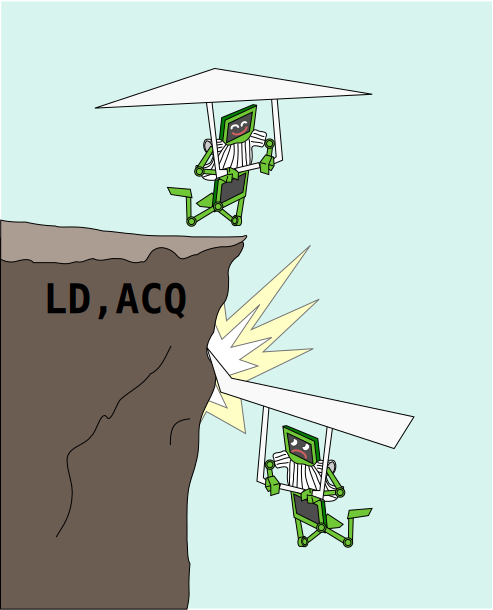
\includegraphics{cartoons/r-2014-LD-ACQ}}
\end{center}
\caption{Half Memory Barrier}
\ContributedBy{Figure}{fig:app:whymb:Half Memory Barrier}{Melissa Brossard}
\end{figure}

These half-memory fences are useful for critical sections, since
it is safe to push operations into a critical section, but can be
fatal to allow them to bleed out.
However, as one of the only CPUs with this property,\footnote{
	ARMv8 has recently added load-acquire and store-release instructions.}
IA64 defines
Linux's semantics of memory ordering associated with lock acquisition
and release.

The IA64 {\tt mf} instruction is used for the {\tt smp\_rmb()},
{\tt smp\_mb()}, and {\tt smp\_wmb()} primitives in the Linux kernel.
Oh, and despite rumors to the contrary, the ``mf'' mnemonic really
does stand for ``memory fence''.

Finally, IA64 offers a global total order for ``release'' operations,
including the ``mf'' instruction.
This provides the notion of transitivity, where if a given code fragment
sees a given access as having happened, any later code fragment will
also see that earlier access as having happened.
Assuming, that is, that all the code fragments involved correctly use
memory barriers.

\subsection{MIPS}

The MIPS memory model~\cite[Table 6.6]{MIPSvII-A-2015}
appears to resemble that of ARM, IA64, and Power,
being weakly ordered by default, but respecting dependencies.
MIPS has a wide variety of memory-barrier instructions, but ties them
not to hardware considerations, but rather to the use cases provided
by the Linux kernel and the C++11 standard~\cite{RichardSmith2015N4527}
in a manner similar to the ARM64 additions:

\begin{description}
\item[SYNC]
	Full barrier for a number of hardware operations in addition
	to memory references.
\item[SYNC\_WMB]
	Write memory barrier, which can be used to implement the
	\co{smp_wmb()} primitive in the Linux kernel.
\item[SYNC\_MB]
	Full memory barrier, but only for memory operations.
	This may be used to implement the Linux-kernel \co{smp_mb()}
	and the C++ \co{atomic_thread_fence(memory_order_seq_cst)}.
\item[SYNC\_ACQUIRE]
	Acquire memory barrier, which may be used to implement the
	Linux-kernel \co{smp_load_acquire()} and the C++
	\co{atomic_load_explicit(..., memory_order_acquire)}.
\item[SYNC\_RELEASE]
	Release memory barrier, which may be used to implement the
	Linux-kernel \co{smp_store_release()} and the C++
	\co{atomic_store_explicit(..., memory_order_release)}.
\item[SYNC\_RMB]
	Read memory barrier, which can be used to implement the
	\co{smp_rmb()} primitive in the Linux kernel.
\end{description}

Informal discussions with MIPS architects indicates that MIPS has a
definition of transitivity or cumulativity similar to that of
ARM and Power.
However, it appears that different MIPS implementations can have
different memory-ordering properties, so it is important to consult
the documentation for the specific MIPS implementation you are using.

\subsection{PA-RISC}

Although the PA-RISC architecture permits full reordering of loads and
stores, actual CPUs run fully ordered~\cite{GerryKane96a}.
This means that the Linux kernel's memory-ordering primitives generate
no code, however, they do use the gcc {\tt memory} attribute to disable
compiler optimizations that would reorder code across the memory
barrier.

\subsection{POWER / PowerPC}
\label{sec:app:whymb:POWER / PowerPC}

The POWER and PowerPC\textsuperscript{\textregistered}
CPU families have a wide variety of memory-barrier
instructions~\cite{PowerPC94,MichaelLyons02a}:
\begin{enumerate}
\item	{\tt sync} causes all preceding operations to {\em appear to have}
	completed before any subsequent operations are started.
	This instruction is therefore quite expensive.
\item	{\tt lwsync} (light-weight sync) orders loads with respect to
	subsequent loads and stores, and also orders stores.
	However, it does {\em not} order stores with respect to subsequent
	loads.
	Interestingly enough, the {\tt lwsync} instruction enforces
	the same ordering as does zSeries, and coincidentally,
	SPARC TSO.
	The \co{lwsync} instruction may be used to implement
	load-acquire and store-release operations.
\item	{\tt eieio} (enforce in-order execution of I/O, in case you
	were wondering) causes all preceding cacheable stores to appear
	to have completed before all subsequent stores.
	However, stores to cacheable memory are ordered separately from
	stores to non-cacheable memory, which means that {\tt eieio}
	will not force an MMIO store to precede a spinlock release.
\item	{\tt isync} forces all preceding instructions to appear to have
	completed before any subsequent instructions start execution.
	This means that the preceding instructions must have progressed
	far enough that any traps they might generate have either happened
	or are guaranteed not to happen, and that any side-effects of
	these instructions (for example, page-table changes) are seen by the
	subsequent instructions.
\end{enumerate}

Unfortunately, none of these instructions line up exactly with Linux's
{\tt wmb()} primitive, which requires {\em all} stores to be ordered,
but does not require the other high-overhead actions of the {\tt sync}
instruction.
But there is no choice: ppc64 versions of {\tt wmb()} and {\tt mb()} are
defined to be the heavyweight {\tt sync} instruction.
However, Linux's {\tt smp\_wmb()} instruction is never used for MMIO
(since a driver must carefully order MMIOs in UP as well as
SMP kernels, after all), so it is defined to be the lighter weight
{\tt eieio} instruction.
This instruction may well be unique in having a five-vowel mnemonic.
The {\tt smp\_mb()} instruction is also defined to be the {\tt sync}
instruction, but both {\tt smp\_rmb()} and {\tt rmb()} are defined to
be the lighter-weight {\tt lwsync} instruction.

Power features ``cumulativity'', which can be used to obtain
transitivity.
When used properly, any code seeing the results of an earlier
code fragment will also see the accesses that this earlier code
fragment itself saw.
Much more detail is available from
McKenney and Silvera~\cite{PaulEMcKenneyN2745r2009}.

Power respects control dependencies in much the same way that ARM
does, with the exception that the Power \co{isync} instruction
is substituted for the ARM \co{ISB} instruction.

Many members of the POWER architecture have incoherent instruction
caches, so that a store to memory will not necessarily be reflected
in the instruction cache.
Thankfully, few people write self-modifying code these days, but JITs
and compilers do it all the time.
Furthermore, recompiling a recently run program looks just like
self-modifying code from the CPU's viewpoint.
The {\tt icbi} instruction (instruction cache block invalidate)
invalidates a specified cache line from
the instruction cache, and may be used in these situations.

\subsection{SPARC RMO, PSO, and TSO}

Solaris on SPARC uses TSO (total-store order), as does Linux when built for
the ``sparc'' 32-bit architecture.
However, a 64-bit Linux kernel (the ``sparc64'' architecture)
runs SPARC in RMO (relaxed-memory order) mode~\cite{SPARC94}.
The SPARC architecture also offers an intermediate PSO (partial store
order).
Any program that runs in RMO will also run in either PSO or TSO, and similarly,
a program that runs in PSO will also run in TSO.
Moving a shared-memory parallel program in the other direction may
require careful insertion of memory barriers, although, as noted earlier,
programs that make standard use of synchronization primitives need not
worry about memory barriers.

SPARC has a very flexible memory-barrier instruction~\cite{SPARC94}
that permits fine-grained control of ordering:
\begin{itemize}
\item	{\tt StoreStore}: order preceding stores before subsequent stores.
	(This option is used by the Linux {\tt smp\_wmb()} primitive.)
\item	{\tt LoadStore}: order preceding loads before subsequent stores.
\item	{\tt StoreLoad}: order preceding stores before subsequent loads.
\item	{\tt LoadLoad}: order preceding loads before subsequent loads.
	(This option is used by the Linux {\tt smp\_rmb()} primitive.)
\item	{\tt Sync}: fully complete all preceding operations before starting
	any subsequent operations.
\item	{\tt MemIssue}: complete preceding memory operations before subsequent
	memory operations, important for some instances of memory-mapped
	I/O.
\item	{\tt Lookaside}: same as MemIssue, but only applies to preceding stores
	and subsequent loads, and even then only for stores and loads that
	access the same memory location.
\end{itemize}

The Linux {\tt smp\_mb()} primitive uses the first four options together,
as in
{\tt membar \#LoadLoad | \#LoadStore | \#StoreStore | \#StoreLoad},
thus fully ordering memory operations.

So, why is {\tt membar \#MemIssue} needed?
Because a {\tt membar \#StoreLoad} could permit a subsequent
load to get its value from a write buffer, which would be
disastrous if the write was to an MMIO register that induced side effects
on the value to be read.
In contrast, {\tt membar \#MemIssue} would wait until the write buffers
were flushed before permitting the loads to execute,
thereby ensuring that the load actually gets its value from the MMIO register.
Drivers could instead use {\tt membar \#Sync}, but the lighter-weight
{\tt membar \#MemIssue} is preferred in cases where the additional function
of the more-expensive {\tt membar \#Sync} are not required.

The {\tt membar \#Lookaside} is a lighter-weight version of
{\tt membar \#MemIssue}, which is useful when writing to a given MMIO register
affects the value that will next be read from that register.
However, the heavier-weight {\tt membar \#MemIssue} must be used when
a write to a given MMIO register affects the value that will next be
read from {\em some other} MMIO register.

It is not clear why SPARC does not define {\tt wmb()} to be
{\tt membar \#MemIssue} and {\tt smb\_wmb()} to be
{\tt membar \#StoreStore},
as the current definitions seem vulnerable to bugs in some drivers.
It is quite possible that all the SPARC CPUs that Linux runs on
implement a more conservative memory-ordering model than the architecture
would permit.

SPARC requires a {\tt flush} instruction be used between the time that
an instruction is stored and executed~\cite{SPARC94}.
This is needed to flush any prior value for that location from
the SPARC's instruction cache.
Note that {\tt flush} takes an address, and will flush only that address
from the instruction cache.
On SMP systems, all CPUs' caches are flushed, but there is no
convenient way to determine when the off-CPU flushes complete,
though there is a reference to an implementation note.

\subsection{x86}

Since the x86 CPUs provide ``process ordering'' so that all CPUs agree
on the order of a given CPU's writes to memory, the {\tt smp\_wmb()} primitive
is a no-op for the CPU~\cite{IntelXeonV3-96a}.
However, a compiler directive is required to
prevent the compiler from performing optimizations that would result
in reordering across the {\tt smp\_wmb()} primitive.

On the other hand, x86 CPUs have traditionally given
no ordering guarantees for loads, so
the {\tt smp\_mb()} and {\tt smp\_rmb()} primitives expand to {\tt lock;addl}.
This atomic instruction acts as a barrier to both loads and stores.

Intel has also published a memory model for
x86~\cite{Intelx86MemoryOrdering2007}.
It turns out that Intel's actual CPUs enforced tighter ordering than
was claimed in the previous specifications, so this model is in effect
simply mandating the earlier de-facto behavior.
Even more recently, Intel published an updated memory model for
x86~\cite[Section 8.2]{Intel64IA32v3A2011}, which mandates a total global order
for stores, although individual CPUs are still permitted to see their
own stores as having happened earlier than this total global order
would indicate.
This exception to the total ordering is needed to allow important
hardware optimizations involving store buffers.
In addition, memory ordering obeys causality, so that if CPU~0 sees a
store by CPU~1, then CPU~0 is guaranteed to see all stores that CPU~1
saw prior to its store.
Software may use atomic operations to override these hardware optimizations,
which is one reason that atomic operations tend to be more expensive
than their non-atomic counterparts.
This total store order is \emph{not} guaranteed on older processors.

It is also important to note that atomic instructions operating
on a given memory location should all be of the same
size~\cite[Section 8.1.2.2]{Intel64IA32v3A2011}.
For example, if you write a program where one CPU atomically increments
a byte while another CPU executes a 4-byte atomic increment on
that same location, you are on your own.

However, note that some SSE instructions are weakly ordered ({\tt clflush}
and non-temporal move instructions~\cite{IntelXeonV2b-96a}).
CPUs that have SSE can use {\tt mfence} for {\tt smp\_mb()},
{\tt lfence} for {\tt smp\_rmb()}, and {\tt sfence} for {\tt smp\_wmb()}.

A few versions of the x86 CPU have a mode bit that enables out-of-order
stores, and for these CPUs, {\tt smp\_wmb()} must also be defined to
be {\tt lock;addl}.

Although newer x86 implementations accommodate self-modifying code
without any special instructions, to be fully compatible with
past and potential future x86 implementations, a given CPU must
execute a jump instruction or a serializing instruction (e.g., \co{cpuid})
between modifying the code and executing
it~\cite[Section 8.1.3]{Intel64IA32v3A2011}.

\subsection{zSeries}

The zSeries machines make up the IBM\textsuperscript{\texttrademark}
mainframe family, previously
known as the 360, 370, and 390~\cite{IBMzSeries04a}.
Parallelism came late to zSeries, but given that these mainframes first
shipped in the mid 1960s, this is not saying much.
The {\tt bcr 15,0} instruction is used for the Linux {\tt smp\_mb()},
{\tt smp\_rmb()}, and {\tt smp\_wmb()} primitives.
It also has comparatively strong memory-ordering semantics, as shown in
Table~\ref{tab:app:whymb:Summary of Memory Ordering}, which should allow the
{\tt smp\_wmb()} primitive to be a {\tt nop} (and by the time you read this,
this change may well have happened).
The table actually understates the situation, as the zSeries memory model
is otherwise sequentially consistent, meaning that all CPUs
will agree on the order of unrelated stores from different CPUs.

As with most CPUs, the zSeries architecture does not guarantee a
cache-coherent instruction stream, hence,
self-modifying code must execute a serializing instruction between updating
the instructions and executing them.
That said, many actual zSeries machines do in fact accommodate self-modifying
code without serializing instructions.
The zSeries instruction set provides a large set of serializing instructions,
including compare-and-swap, some types of branches (for example, the
aforementioned {\tt bcr 15,0} instruction), and test-and-set,
among others.

\section{Are Memory Barriers Forever?}
\label{sec:app:whymb:Are Memory Barriers Forever?}

There have been a number of recent systems that are significantly less
aggressive about out-of-order execution in general and re-ordering
memory references in particular.
Will this trend continue to the point where memory barriers are a thing
of the past?

The argument in favor would cite proposed massively multi-threaded hardware
architectures, so that each thread would wait until memory was ready,
with tens, hundreds, or even thousands of other threads making progress
in the meantime.
In such an architecture, there would be no need for memory barriers,
because a given thread would simply wait for all outstanding operations
to complete before proceeding to the next instruction.
Because there would be potentially thousands of other threads, the
CPU would be completely utilized, so no CPU time would be wasted.

The argument against would cite the extremely limited number of applications
capable of scaling up to a thousand threads, as well as increasingly
severe realtime requirements, which are in the tens of microseconds
for some applications.
The realtime-response requirements are difficult enough to meet as is,
and would be even more difficult to meet given the extremely low
single-threaded throughput implied by the massive multi-threaded
scenarios.

Another argument in favor would cite increasingly sophisticated
latency-hiding hardware implementation techniques that might well allow
the CPU to provide the illusion of fully sequentially consistent
execution while still providing almost all of the performance advantages
of out-of-order execution.
A counter-argument would cite the increasingly severe power-efficiency
requirements presented both by battery-operated devices and by
environmental responsibility.

Who is right?
We have no clue, so are preparing to live with either scenario.

\section{Advice to Hardware Designers}
\label{sec:app:whymb:Advice to Hardware Designers}

There are any number of things that hardware designers can do
to make the lives of software people difficult.
Here is a list of a few such things that we have encountered in
the past, presented here in the hope that it might help prevent
future such problems:
\begin{enumerate}
\item	I/O devices that ignore cache coherence.

	This charming misfeature can result in DMAs from memory
	missing recent changes to the output buffer, or, just as
	bad, cause input buffers to be overwritten by the contents
	of CPU caches just after the DMA completes.
	To make your system work in face of such misbehavior,
	you must carefully flush the CPU caches of any location
	in any DMA buffer before presenting that buffer to the
	I/O device.
	Similarly, you need to flush the CPU caches of any location
	in any DMA buffer after DMA to that buffer completes.
	And even then, you need to be \emph{very} careful to avoid
	pointer bugs, as even a misplaced read to an input buffer
	can result in corrupting the data input!

\item	External busses that fail to transmit cache-coherence data.

	This is an even more painful variant of the above problem,
	but causes groups of devices---and even memory itself---to
	fail to respect cache coherence.
	It is my painful duty to inform you that as embedded systems
	move to multicore architectures, we will no doubt see a fair
	number of such problems arise.
	Hopefully these problems will clear up by the year 2015.

\item	Device interrupts that ignore cache coherence.

	This might sound innocent enough --- after all, interrupts
	aren't memory references, are they?
	But imagine a CPU with a split cache, one bank of which is
	extremely busy, therefore holding onto the last cacheline
	of the input buffer.
	If the corresponding I/O-complete interrupt reaches this
	CPU, then that CPU's memory reference to the last cache
	line of the buffer could return old data, again resulting
	in data corruption, but in a form that will be invisible
	in a later crash dump.
	By the time the system gets around to dumping the offending
	input buffer, the DMA will most likely have completed.

\item	Inter-processor interrupts (IPIs) that ignore cache coherence.

	This can be problematic if the IPI reaches its destination
	before all of the cache lines in the corresponding message
	buffer have been committed to memory.

\item	Context switches that get ahead of cache coherence.

	If memory accesses can complete too wildly out of order,
	then context switches can be quite harrowing.
	If the task flits from one CPU to another before all the
	memory accesses visible to the source CPU make it to the
	destination CPU, then the task could easily see the corresponding
	variables revert to prior values, which can fatally confuse
	most algorithms.

\item	Overly kind simulators and emulators.

	It is difficult to write simulators or emulators that force
	memory re-ordering, so software that runs just fine in
	these environments can get a nasty surprise when it first
	runs on the real hardware.
	Unfortunately, it is still the rule that the hardware is more
	devious than are the simulators and emulators, but we hope that
	this situation changes.
\end{enumerate}

Again, we encourage hardware designers to avoid these practices!
